\documentclass{OptiFlow}

\usepackage[utf8]{inputenc}
\usepackage[T1]{fontenc}
\usepackage{textcomp}
\usepackage{amsmath, amssymb}
\usepackage{mdframed}
\usepackage{pgfplots}
\usepackage{import}
\usepackage{mathrsfs}
\usepackage{xifthen}
\usepackage{float}
\usepackage{nicematrix}
\usepackage{pdfpages}
\usepackage{tcolorbox}
\usepackage{transparent}
\pgfplotsset{compat=1.18}
\usepackage{tikz}
\usetikzlibrary{shapes.misc}
\newtheorem{theorem}{Theorem}{}
\newtheorem{corollary}{Corollary}{}
\newtheorem{remark}{Remark}{}

\usetikzlibrary{arrows, arrows.meta}

\tikzset{cross/.style={cross out, draw=black, minimum size=2*(#1-\pgflinewidth), inner sep=0pt, outer sep=0pt, style = ultra thick},
%default radius will be 1pt. 
cross/.default={5pt}}

% figure support
\usepackage{import}
\usepackage{xifthen}
\usepackage{collectbox}
\usepackage{enumerate}
\usepackage{amsfonts}
\pdfminorversion=7
\usepackage{pdfpages}
\usepackage{transparent}
\newcommand{\incfig}[1]{%
	\def\svgwidth{\columnwidth}
	\import{./figures/}{#1.pdf_tex}
}
\usepackage{fancyhdr}

\begin{document}

\supertitle{HackUPC 2023}

\title{Optimizing Supply Chain Robustness}

\author{\au{Nathaniel Mitrani $^{1}$}, \au{Alex Serrano $^{2}$}, \au{Jan Tarrats $^{3}$}}

\address{\add{1}{Mathematics and Data Science and Engineering, UPC, Barcelona, Spain}
\add{2}{Mathematics and Data Science and Engineering, UPC, Barcelona, Spain}
\add{3}{Mathematics and Computer Engineering, UPC, Barcelona, Spain}
}

\begin{abstract}
In this project, we propose a novel manner to optimize the robustness of a supply chain through stochastic modeling of its disruptions.
\end{abstract}

\maketitle

\section{Introduction}\label{sec1}
Supply chain robustness is of paramount importance for businesses, as it not only ensures operational continuity 
but also provides significant financial benefits. By investing in robust supply chains, 
companies can minimize disruptions and associated costs, such as production delays, inventory shortages, 
and customer dissatisfaction. A resilient supply chain reduces the likelihood of stockouts, thereby avoiding revenue losses and preserving customer loyalty. 
Ultimately, supply chain robustness directly contributes to a company's bottom line and long-term profitability.

\vspace{5mm}

\section{Problem Statement}\label{sec2}
We have a certain sales forecast, $s_t$, and a given storage capacity, $c_t$.
We assume that when demanding a certain amount of units in inventory, $q_t$, we model the resultant amount of units in inventory
as a normal distribution ($\Phi\left( x \right) $) with mean $q_t$ and variance $\sigma^2$, a fixed parameter based on advanced studies about the state of the supply chain and its disruptions.
With the help of cost functions that help us penalize both the storage ($c\left( n \right) $) and the penalization of the stockout ($\delta_n$), we want to find the optimal amount of units to order, $q_t$, in order to minimize the expected cost of the supply chain.
These functions, decided by the company, are hereby assumed to be linear, with a fixed cost and a variable cost per unit, however,
the model can be easily adapted to other types of functions. (See figure \ref{fig})

\vspace{10mm}

\begin{figure}[ht]
	\centering
	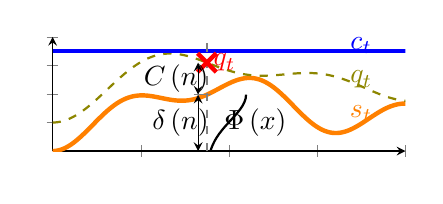
\begin{tikzpicture}[font=\sffamily,
declare function={gauss(\x,\y,\z)=1/(\y*sqrt(2*pi))*exp(-((\x-\z)^2)/(2*\y^2));}]

		\begin{axis}[
			width=0.5\textwidth,
			height = 0.25\textwidth,
			xmin= 0, xmax=4,
			ymin= 0, ymax = 4,
			axis lines = middle,
			yticklabels={,,},
			xticklabels={,,},
		]
		\addplot[domain=0:4, samples=1000, color = orange, style = ultra thick]{(sin(deg(x)))^2+(sin(2*deg(x)))^2+ (sin(0.7*deg(x)))^2};
		\addplot[domain=0:4, samples=1000, color = olive, style = thick, dashed]{(sin(deg(x)))^2+(sin(1.5*deg(x)))^2+ (sin(0.7*deg(x)))^2+1};
		\addplot[domain=0:4, samples=1000, color = blue, style = ultra thick]{3.5};

		\addplot[thick, samples=50, smooth,domain=0:6,gray, dashed] coordinates {(1.75,0)(1.75,4)};

		\draw (1.75,3.097) node[cross, red]{};
		\draw[>=stealth, thin, <->] (1.65,0) -- (1.65,1.976);
		\draw[>=stealth, <->] (1.65,1.976) -- (1.65,3.097);
		
		\draw[gray] (1.6,1.976) -- (1.8,1.976);

		
		\addplot [domain=-3:0, thick] ({1.75+gauss(x,0.9,0)},1.976+x);

		\draw[red] (1.95, 3.097) node {$q_t$};
		\draw (1.4, 2.5365) node {$C\left( n \right) $};i
		\draw (1.45, 0.988) node {$\delta\left( n \right) $};
		\draw[orange] (3.5, 1.3) node {$s_t$};
		\draw[olive] (3.5, 2.5) node {$q_t$};
		\draw[blue] (3.5, 3.7) node {$c_t$};
		\draw[black] (2.3,1) node {$\Phi\left( x \right) $};
	\end{axis}
	\end{tikzpicture}
	\caption{Optimization model}
	\label{fig}
\end{figure}	

\newpage
\section{Functions Definitions}
\subsection{Storage Cost Function}
We hereby define the storage cost function as follows:

$\text{ }$ 

\hfill\begin{minipage}{\dimexpr0.5\textwidth-1cm}
	\begin{itemize}
	\item $c$: fixed storage cost per unit
	\item $K_1$: administrative cost per order
	\item $n$: difference between the amount of units demanded in inventory and the amount of units forecasted to be sold
\end{itemize}
\end{minipage}


\begin{align*}
	&c, K_1 \in \mathbb{R}\\
	&n \equiv q_t - s_t\\
	&C\left( n \right) =  \begin{cases}
		0 \text{\qquad} &n \le  0\\
		c\cdot n +K_1 \text{\qquad} &n>0
	\end{cases}  
.\end{align*}

\subsection{Penalization Cost Function}
We hereby define the penalization cost function as follows, this is the cost of having a stockout:

$\text{ }$

\hfill\begin{minipage}{\dimexpr0.5\textwidth-1cm}
\begin{itemize}
	\item $d$: fixed cost per unit
	\item $K_2$: administrative cost per order
	\item $n$: difference between the amount of units forecasted to be sold and the amount of units demanded in inventory
\end{itemize}
\end{minipage}

\begin{align*}
	&d,K_2 \in  \mathbb{R}\\
	&n \equiv s_t - q_t\\
	&\delta\left( n \right) = \begin{cases}
		0 \text{\qquad} &n \le  0\\
		d\cdot n + K_2 \text{\qquad} &n > 0
	\end{cases}
.\end{align*}

\subsection{Normal Density Function}
We hereby define the normal density function as follows:

$\text{ }$

\hfill\begin{minipage}{\dimexpr0.5\textwidth-1cm}
\begin{itemize}
	\item $\mu \equiv q_t$: mean of the normal distribution, parameter to be optimized
	\item $\sigma^2$: variance of the normal distribution, fixed parameter
	\item $x$: value of the random variable
\end{itemize}
\end{minipage}

\begin{align*}
	&\sigma \in \mathbb{R}\\
	&\Phi_{\mu=q_t, \sigma^2}\left( x \right)   = \frac{1}{\sigma \sqrt{2\pi} }e^{- \frac{\left( x-\mu \right) ^2}{2 \sigma^2}}
.\end{align*}


\subsection{Loss function}
We assumed that given a demanded amount of units in inventory, $q_t$, the resultant amount of units in inventory
follows a normal distribution with mean $q_t$ and variance $\sigma^2$, that is only on the positive real numbers (and therefore scaled).
We must penalize two things, the storage and the penalization of the stockout, therefore, we define the loss function as 
the expected value of the sum of the storage cost function and the penalization cost function, as follows:

\subsubsection{Theoretical}
\begin{align*}
	loss\left( q_t \right)   = \int_{s_t}^{q_t} &c\left( z,s_t \right) \cdot \Phi_{\mu, \sigma^2}\left( z \right) dz+ \\
										&+ \int_{0}^{s_t} \delta\left( z,s_t \right)\cdot \Phi_{\mu, \sigma^2}\left( z \right) dz  
.\end{align*}

As we are solving this problem numerically, and depending on the decided cost 
functions, the problem does not admit a closed form solution, therefore, we must approximate the loss function.
To do so, we will use the following approximation:

\subsubsection{Aproximation}
\begin{align*}
	loss\left( q_t \right)  \approx \sum_{i = s_t}^{q_t+step} &c\left( i,s_t \right) \cdot \Phi_{\mu, \sigma^2}\left( i, q_t \right) + \\
	&+ \sum_{j = 0}^{s_t + step} \delta\left( j,s_t \right) \cdot \Phi_{\mu, \sigma^2}\left( j,q_t \right) 
.\end{align*}

\section{Problem Goal}
Therefore, our problem can be mathematically stated as follows:
\subsection{Theoretical}
\vspace{-5mm}
\begin{align*}
	&\underset{q_t}{\text{argmin}} \text{\qquad \qquad}loss\left( q_t \right)\\ 
	&\text{subject to}
		\text{\qquad\quad} 0 \le q_t \le  c_t \text{\qquad} t = 1,\ldots,T
.\end{align*}

This allows us to find the optimal amount of units to order, $q_t*$, in order to minimize the expected cost of the supply chain,
thus optimizing the supply chain robustness by preventing stockouts and minimizing storage costs.

\section{Problem Solution: Numerical Optimization}
As we are solving this problem numerically, we must define a numerical optimization method.
We will use a grid search of the $\mu \equiv q_t$ parameter, with a step of 1, and then we will use that as an approximation of the optimal value of $q_t$.
This has the advantage of being numerically simple, and it is also easy to implement in a computer program, and its speed can be 
regulated by changing the step size, however sacrificing the accuracy of the prediction.

\section{Example solution: product 25662}
We will now show an example of the solution of the problem for a certain product, 25662.
We will assume that the capacity is the maximum of the inventory in the time frame we are looking at, and use the reported sales 
as the supposed sales forecast.

\begin{figure}[htpb]
	\centering
	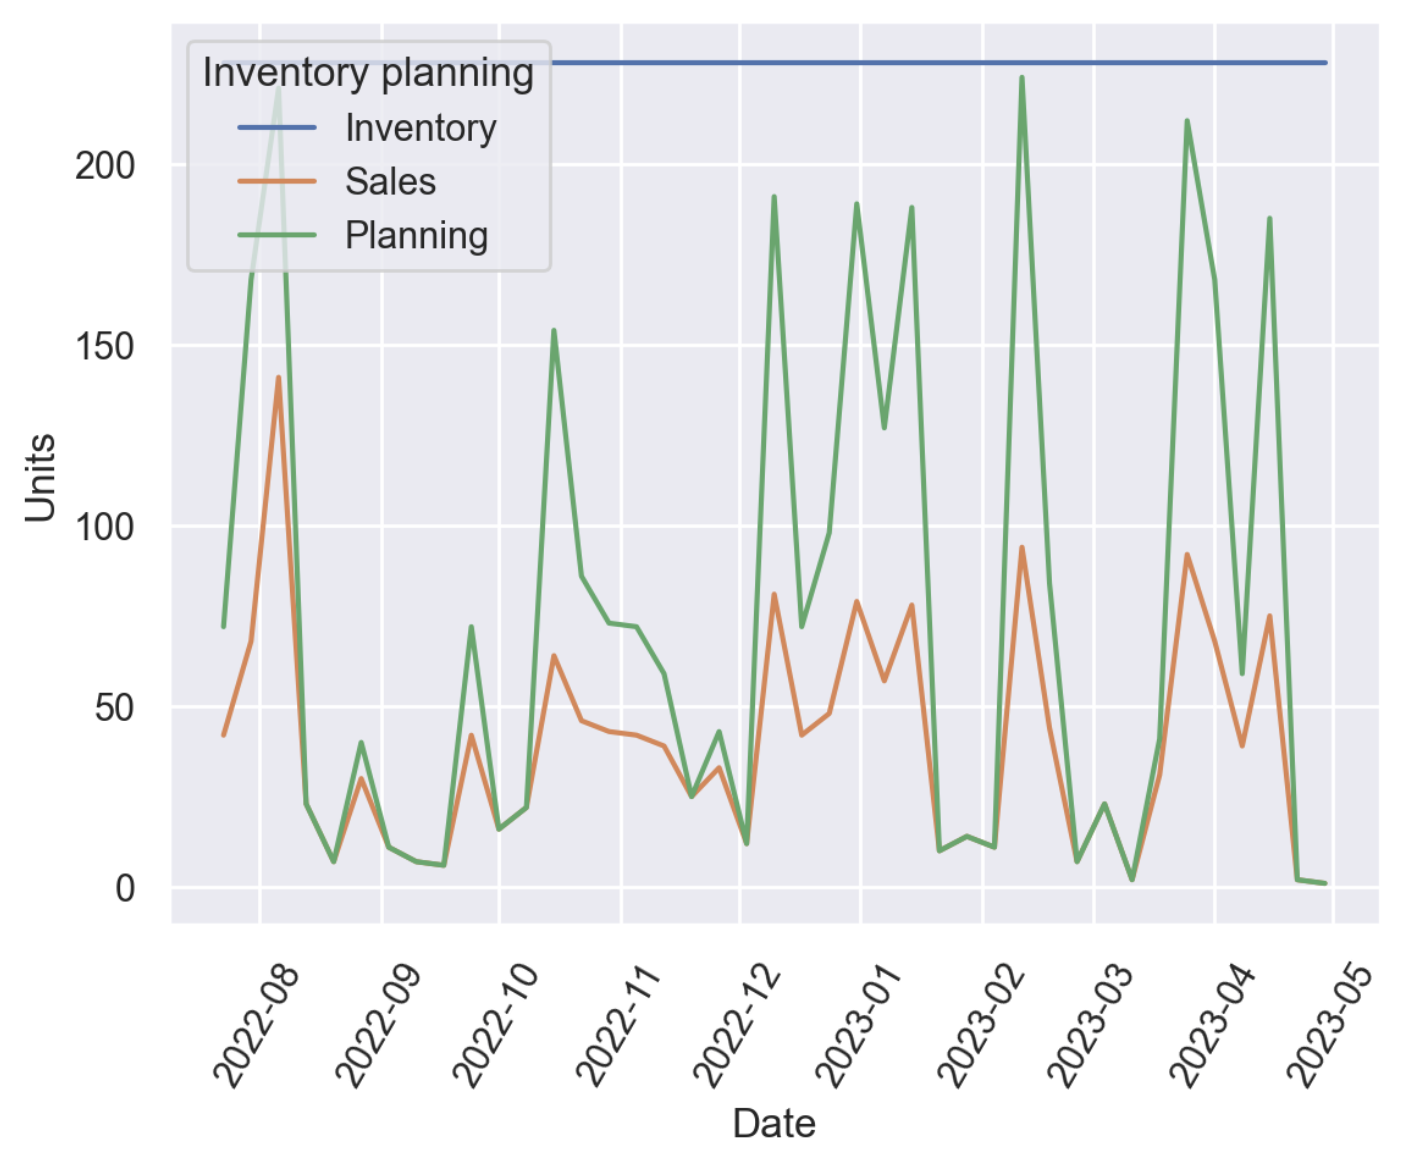
\includegraphics[width=0.4\textwidth]{25662.png}
	\caption{Inventory Planning 25662}
	\label{fig:graf1}
\end{figure}

As we can see in figure \ref{fig:graf1}, the optimal amount of units to order 
fluctuates in values over the forecasted amount of sales, and it is always below the capacity of the warehouse.
This is because the cost of having a stockout is much higher than the cost of having a surplus of units in inventory,
and therefore, the optimal solution is to order more units than the forecasted amount of sales, in order to prevent stockouts.
It is noteworthy that the optimal amount of units to order is not constant over time, and it fluctuates depending on the
forecasted amount of sales, and in other assumptions on the capacity of the warehouse. Not only that,
but here the demand does not stress the capacity of the warehouse, and therefore, the optimal amount of units to order is always much below the capacity of the warehouse.

\section{Example solution: product 7896}
We will now show an example of the solution of the problem for a certain other product, 7896.
We will again assume that the capacity is the maximum of the inventory in the time frame we are looking at, and use the reported sales 
as the supposed sales forecast.

\vspace{-2mm}

\begin{figure}[htpb]
	\centering
	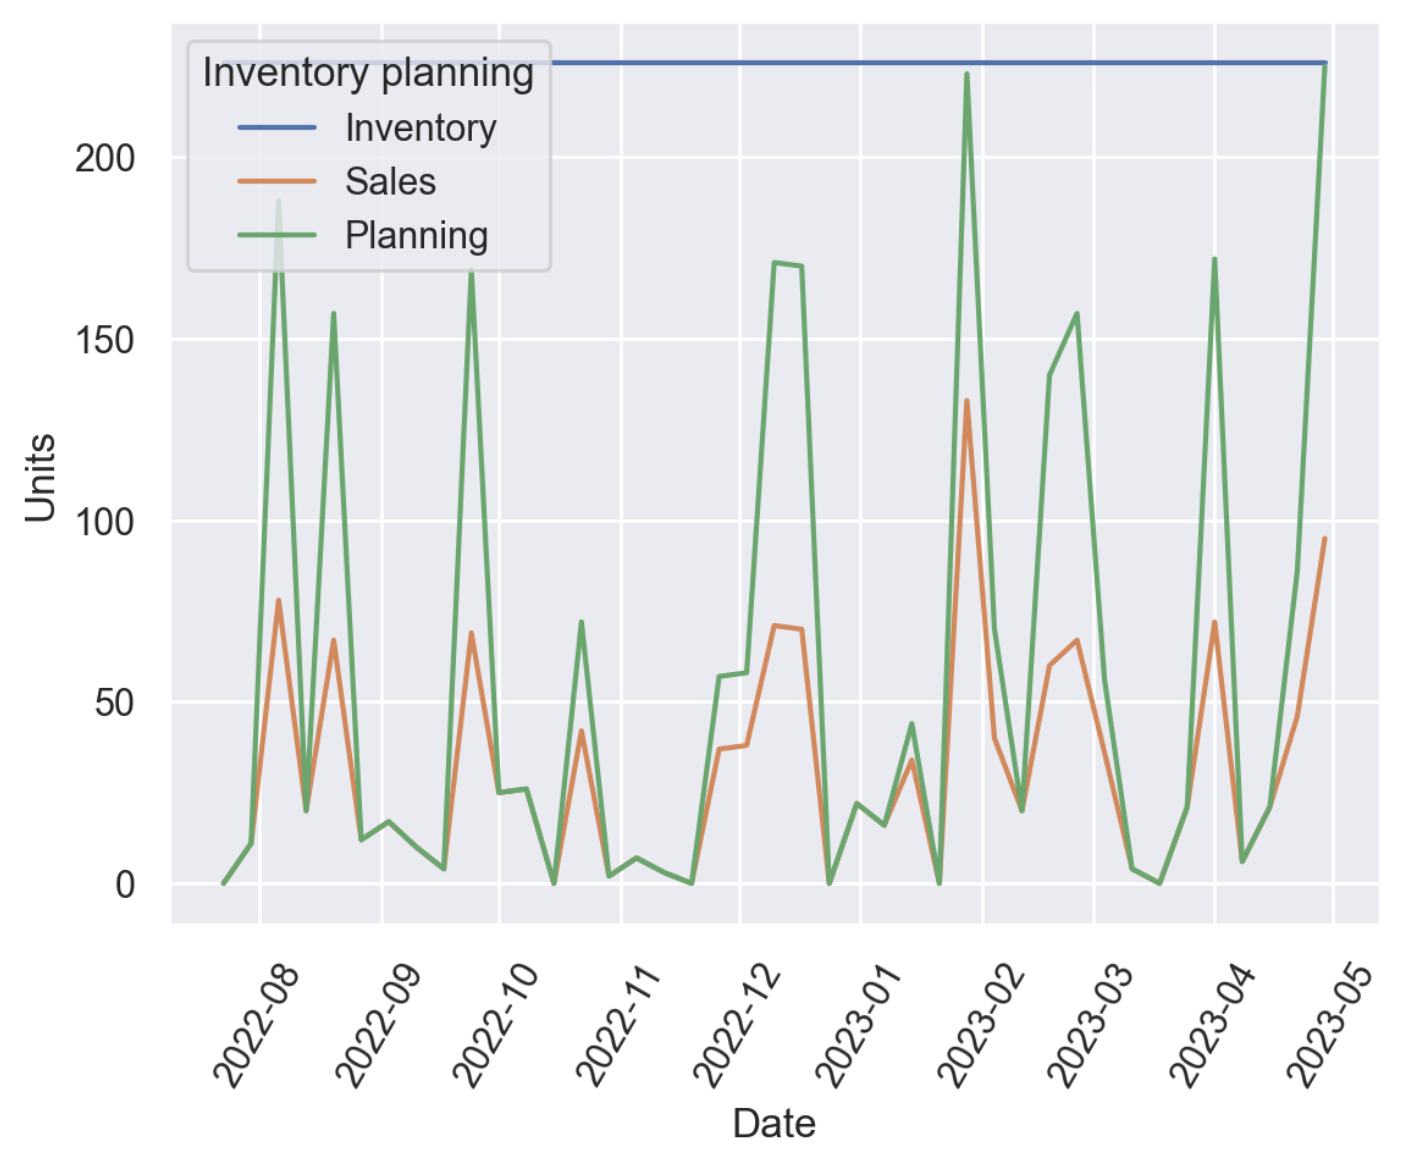
\includegraphics[width=0.4\textwidth]{7896.png}
	\caption{Inventory Planning 7896}
	\label{fig:graf2}
\end{figure}

\vspace{-2mm}

As we can see in figure \ref{fig:graf2}, this case is different from the previous one, as the demand stresses the capacity of the warehouse,
and therefore the optimal amount of units to order is much closer to the capacity of the warehouse, even matching it in the last observation.

\section{Quantification of the robustness of the supply chain: expected profit}
We will now quantify the robustness of the supply chain by calculating the expected profit of the supply chain.
This is computing by substracting the loss function from the forecasted sales (naive approach) to the optimal amount of units to order that we computed.
This value yields XXXX, and if we put out loss function units in USD, this means that we are saving XXXX USD in the supply chain thanks to our optimization model.



\end{document}
